%% right-side equation numbering, 12 point font, print one-sided 
%\documentclass[reqno,12pt,oneside]{report} 
\documentclass[12pt,letterpaper,oneside]{book}

% Use my personal style sheet
%\usepackage{tomf}         

\usepackage{color}
\usepackage{times}
\usepackage{amsmath,amsfonts,amssymb}
\usepackage{amsthm}   % for theorems
%\usepackage{graphics}
\usepackage{graphicx} % This is preferred. %> convert image.png image.eps
\usepackage{comment}

%%%%%%%%%%%%%%%%%%%%%%%%%%%%%%%%%%%%%%%%%%%%%%%%%%%%%%%%%%%%%%%%%%%%%%%%%%%%%%%

% Various theorem environments. All of the following have the same numbering
% system as theorem.

\theoremstyle{plain}
\newtheorem{theorem}{Theorem}
\newtheorem{prop}[theorem]{Proposition}
\newtheorem{corollary}[theorem]{Corollary}
\newtheorem{lemma}[theorem]{Lemma}
\newtheorem{question}[theorem]{Question}
\newtheorem{conjecture}[theorem]{Conjecture}
\newtheorem{assumption}[theorem]{Assumption}

\theoremstyle{definition}
\newtheorem{definition}[theorem]{Definition}
\newtheorem{notation}[theorem]{Notation}
\newtheorem{condition}[theorem]{Condition}
\newtheorem{example}[theorem]{Example}
\newtheorem{introduction}[theorem]{Introduction}

\theoremstyle{remark}
\newtheorem{remark}[theorem]{Remark}

% Numbers theorems "x.y" where x is the section number, y is the theorem number
\numberwithin{theorem}{chapter}     

%%%%%%%%%%%%%%%%%%%%%%%%%%%%%%%%%%%%%%%%%%%%%%%%%%%%%%%%%%%%%%%%%%%%%%%%%%%%%%%
\usepackage{listings}

\definecolor{dkgreen}{rgb}{0,0.6,0}
\definecolor{gray}{rgb}{0.5,0.5,0.5}
\definecolor{mauve}{rgb}{0.58,0,0.82}

\lstset{ 
  backgroundcolor=\color{white},  % choose the background color; \usepackage{[x]color} 
  basicstyle=\footnotesize\ttfamily,       % the size of the fonts that are used for the code
  breakatwhitespace=false,        % sets if automatic breaks should only happen at whitespace
  breaklines=true,                % sets automatic line breaking
  captionpos=b,                   % sets the caption-position to bottom
  commentstyle=\color{dkgreen},   % comment style
  deletekeywords={...},           % if you want to delete keywords from the given language
  escapeinside={\%*}{*)},         % if you want to add LaTeX within your code
  %extendedchar=true,              % lets you use non-ASCII characters; for 8-bits encodings
  frame=single,                   % adds a frame around the code
  keywordstyle=\color{blue},      % keyword style
  language=Python,                % the language of the code
  morekeywords={*,...},           % if you want to add more keywords to the set
  numbers=none,                   % location of line-numbers; (none, left, right)
  numbersep=5pt,                  % how far the line-numbers are from the code
  numberstyle=\tiny\color{gray},  % the style that is used for the line-numbers
  rulecolor=\color{black},        % if not set, the frame-color may be changed on line-breaks  
  showstringspaces=false,         % underline spaces within strings only
  showtabs=false,                 % show tabs within strings adding particular underscores
  stepnumber=2,                   % the step between two line-numbers. If 1, each line numbered
  stringstyle=\color{mauve},      % string literal style
  tabsize=2,                      % sets default tabsize to 2 spaces
  title=\lstname                  % show the filename of files included with \lstinputlisting; 
}

%%%%%%%%%%%%%%%%%%%%%%%%%%%%%%%%%%%%%%%%%%%%%%%%%%%%%%%%%%%%%%%%%%%%%%%%%%%%%%

\usepackage{tikz}
\usetikzlibrary{shapes}
\newcommand*\circled[1]{\tikz[baseline=(char.base)]{
            \node[shape=circle,draw,inner sep=2pt] (char) {#1};}}
\newcommand*\squared[1]{\tikz[baseline=(char.base)]{
            \node[shape=rectangle,draw,inner sep=4pt] (char) {#1};}}
\newcommand*\triangled[1]{\tikz[baseline=(char.base)]{
            \node[shape=regular polygon,regular polygon sides=3,draw,inner sep=0pt] (char) {#1};}}
%% Example: \circled{1} \squared{2} \triangled{3}

%%%%%%%%%%%%%%%%%%%%%%%%%%%%%%%%%%%%%%%%%%%%%%%%%%%%%%%%%%%%%%%%%%%%%%%%%%%%%%

%% This command creates a box marked ``To Do'' around text.
%% To use type \todo{  insert text here  }.

\newcommand{\todo}[1]{\vspace{5 mm}\par \noindent
\marginpar{\textsc{To Do}}
\framebox{\begin{minipage}[c]{0.95 \textwidth}
\tt\begin{center} #1 \end{center}\end{minipage}}\vspace{5 mm}\par}

\def\startabstractpage#1{% This formats the optional in-dissertation abstract - jg
 \newpage
 \setcounter{page}{1}   % -- begin with "i" TRF
 \addcontentsline{toc}{chapter}{ABSTRACT}
 \@restonecolfalse\if@twocolumn\@restonecoltrue\onecolumn\fi
 \hbox{ }
 \twoinmar
 \centerline{ABSTRACT}
 \vspace{0.4in}
 \noindent #1
 \vspace{0.25in}\\
}

%%%%%%%%%%%%%%%%%%%%%%%%%%%%%%%%%%%%%%%%%%%%%%%%%%%%%%%%%%%%%%%%%%%%%%%%%%%%%%%%%%%%%%%%%%

\begin {document}

%%%%%%%%%%%%%%%%%%%%%%%%%%%%%%%%%%%%%%%%%%%%%%%%%%%%%%%%%%%%%%%%%%%%%%%%%%%%%%%%%%%%%%%%%%

% Page numbering. If you don't include a frontispiece or copyright
% page, you'll need to change this for two-sided printing.
\makeatletter
\if@twoside \setcounter{page}{4} \else \setcounter{page}{1} \fi
\makeatother

% Abstract
%\startabstractpage{\input{abstract}}

% Table of contents, list of figures, etc.
%\tableofcontents     % Required
%\listoftables        % Required if there is more than one table
%\listoffigures       % Required if there is more than one figure
%\listofmaps          % Required if there is more than one map
%\listofappendices    % Required if there is more than one appendix
%\listofabbreviations % Optional. Abbreviations should be stored in a file named abbr.tex

% Optional in-dissertation Abstract Page
%\startabstractpage{The Title of Your Dissertation}{Your Name}{Chair: Albert Einstein}
%\input{Abstract/Abstract}
%\label{Abstract}

%%%%%%%%%%%%%%%%%%%%%%%%%%%%%%%%%%%%%%%%%%%%%%%%%%%%%%%%%%%%%%%%%%%%%%%%%%%%%%%%%%%%%%%%%%
%\startthechapters 
% The individual files for each of the chapters are put here.
% Save each chapter of your thesis to a seperate tex file
% and then use the \input command to include this file in your
% thesis.  For instance you can save a file to "intro.tex" and 
% then type \input{intro}. 
%%%%%%%%%%%%%%%%%%%%%%%%%%%%%%%%%%%%%%%%%%%%%%%%%%%%%%%%%%%%%%%%%%%%%%%%%%%%%%%%%%%%%%%%%%
% use \input   for non-page-break % and \include for page-break

%\chapter{Introduction}
%figure \ref{fig:gaussian}. Here, no presumption is yet made about the kind of distribution for the source (random) variable $X$. 

\begin{figure}
  \centering
  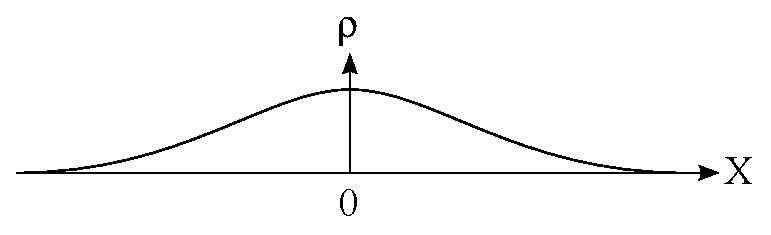
\includegraphics{Images/gaussian.eps}
  \caption[Distribution of source variable $X$]
          {Distribution of source variable $X$}
  \label{fig:gaussian}
\end{figure}

Following Dineen \cite{dineen00}

\chapter{One Dimension}
\section{One Dimension}

This section covers the computing of functions of a single random variable. The following serve as motivating examples,
\begin{enumerate}
\item $X^2$
\item $log(X)$
\item $\frac{1}{X}$
\item $\frac{1}{log(X^2-X)}$
\item $[X-k]^+ - [X-k]^- \equiv X - k$
\label{example:motivating_examples}
\end{enumerate}

An interesting feature of the last item, known as Put-Call Parity \cite{dineen00}, is that it seems to recover lost information through truncation. If $Z_+ := [X-k]^+$ and $Z_- := [X-k]^-$ then $Z_+$ and $Z_-$ are maximally correlated. In the language of quantum mechanics the two $Z$'s are \emph{maximally entangled}. \todo{find reference}

As a naming convenience it is assumed that $X$ represents a \emph{basic random variable}. A basic random variable is on that is not related to any other random variable within RICO by an explicit function. Conversely the label $Z$ refers to a random variable that is functionally related to some $X$ via an explicit function $f$ such that $Z = f(X)$. When more than one function of $X$ is needed they will be distinguished by subscripting. Since a random variable is defined by its associated cumulative density function RICO requires random variables to be associated with the following computable expressions
\begin{align}
P(Z < k) && P(Z = k)
\label{exp:required_expressions}
\end{align}
for any constant $k$. In order to incorporate functions of random variables into an algorithmic context is it also necessary to be able to compute
\begin{align*}
P(Z_1 < Z_2) && \text{ where } && Z_1 = f_1(X),\: Z_2 = f_2(X)
\end{align*}
Notice that $P(Z_1 < Z_2) = P(Z_1 - Z_2 < 0)$ and that $Z_1 - Z_2$ is itself a random variable. The computable expressions in (\ref{exp:required_expressions}) are sufficient to compute $P(Z_1 < Z_2)$ which may arise in conditional branching statements such as $if(Z_1 < Z_2) \{...\}$. Both branches of an \emph{if} statement may be followed albeit with different associated probabilities. Conditional branching statements will be discussed in a later section.

\subsection{Plotting $Z = f(X)$}

A \emph{continuous} random variable has the property that
\begin{align}
P(X = k) = 0 \;\forall \;k \in \mathcal{D}(X)
\label{prop:conditional_random_variable}
\end{align}
and it assumed by RICO that a continuous random variable has an associated probability density function, $\rho(X)$. The expression $\mathcal{D}(X)$ refers to the support of $X$ which in the continuous case is the domain of the associated probability density function.

A \emph{discrete} random variable has discrete support such that
\begin{align}
P(X = k_i) = p_i \;\forall\;k_i \in K = \{k_1, k_2, \dots, k_n\}
\label{prop:discrete_random_variable}
\end{align}

In general a random variable $X$ may be a mixture of continuous and discretely ditributed probability. In RICO the continuous and discrete aspects of a random variable are represented separately. The continuous aspect of a random variable is more numerically challenging and will be the focus of this section as a special case. 

Notice that the discrete aspect of a random variable cannot be ignored even if an original $X$ is purely continuous. Consider the motivating example, $Z = [X-k]^+$ in (\ref{example:motivating_examples}), transforms a continuous $X$ into a \emph{mixed} continuous/discrete $Z$.

In the next section it is assumed that both $X$ and $Z = f(X)$ are continuous random variables.

\subsubsection{Plotting Continuous $Z = f(X)$}

To plot the probability density function of $Z = f(X)$ it is assumed that a software module will be employed to render the actual graph for the user and that the module requires an array of pairs of points, 
\begin{align}
\{(z_i, h_i)\}_{i=1}^n
\label{exp:graph_list}
\end{align}
where $z_i$ is a point in the support of $Z$ and $h_i = \rho(z_i)$, the probability density of $Z$ at $z_i$. The associated probability density function of $Z$ is denoted $\rho(Z)$. 

To first approximation the values of each $h_i$ are found by choosing a set of partition endpoints 
\begin{align*}
(z_i^p)_{i=1}^n \subset \mathcal{D}(Z)
\end{align*}
so that 
\begin{align*}
z_i \in (z_i^p, z_{i+1}^p)
\end{align*}
and the $h_i$ are approximated as
\begin{align*}
h_i = \frac{p_i}{z_{i+1}^p - z_i^p} && \text{ where } p_i = P(z_i^p < Z < z_{i+1}^p) && i = 1,\dots,n
\end{align*}
A \emph{partition of $Z$} is understood to be a partition of the range of $f(X)$.

\begin{figure}
  \centering
  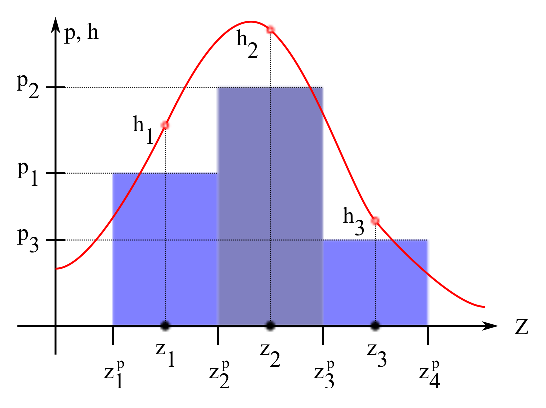
\includegraphics{Images/Zpartition4.eps}
  \caption[Three point Partition of $Z$]
          {Three point Partition of $Z$}
  \label{fig:Zpartition4}
\end{figure}

The relationship between the partition elements is shown in figure \ref{fig:Zpartition4}. Assuming $n \ge 2$ the $z_i^p$ partition points are computed in RICO as midpoints of the $(z_i)_{i=1}^n$ array
\begin{align*}
z_i^p = \begin{cases}
       z_1 - \frac{1}{2}(z_1 + z_2) & \text{ if } i = 1\\
       \frac{1}{2}(z_{i-1} + z_i) & \text{ if } 1 < i \le n\\
       z_n + \frac{1}{2}(z_{n-1} + z_n) & \text{ if } i = n+1\\
      \end{cases}
\end{align*}
Let the associated partition of $Z$ be
\begin{align*}
Z^p =(-\infty, z_1^p, z_2^p, ..., z_{n+1}^p, \infty)
\end{align*}

Since $Z$ is a purely continuous random variable the \emph{partition elements} of $Z^p$ are assumed in RICO to be open intervals. The missing endpoints of the partition elements form a set of probability zero. Let the partition elements of $Z^p$ and associated probability values be indexed as
\begin{align*}
Z_0^p &= (-\infty, z_1^p) && p_0 = P(Z_0^p)\\
Z_i^p &= (z_i^p, z_{i+1}^p) && p_i = P(Z_i^p) && i = 1, \dots, n\\
Z_{n+1}^p &= (z_{n+1}^p, \infty) && p_{n+1} = P(Z_{n+1}^p)
\end{align*}

\subsubsection{Numerical Considerations}

\begin{figure}
  \centering
  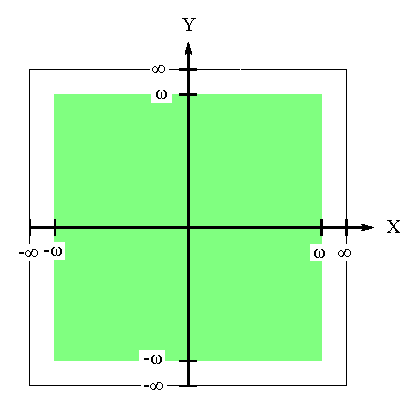
\includegraphics{Images/Quadrants.eps}
  \caption[Fundamental Numeric Domain]
          {Fundamental Numeric Domain}
  \label{fig:Quadrants}
\end{figure}

Numerically, real numbers are represented by a finite number of floating point values. Let $\Omega$ be the largest representable floating point value. Similarly let $\iota$ be the smallest positive floating point value. In RICO, a constant called $\omega$ is defined as
\begin{align}
\omega = min \left\{\Omega, \frac{1}{\iota} \right\}
\label{constant:omega}
\end{align}
and let $\epsilon$ be the smallest numerically representable positive probability value. One purpose for defining $\epsilon$ is so that so-called \emph{thin tailed} probability distribution such as the Gaussian may be represented using a finite support interval as in
\begin{align*}
\mathcal{D}(X) = (X_{min}, X_{max})
\end{align*}
where $-X_{min} = X_{max} \approx 10$, depending on $\epsilon$. The $X_{min}$ and $X_{max}$ satisfy the following relations
\begin{align*}
P(X < X_{min}) \le \epsilon && P(X_{max} < X) \le \epsilon
\end{align*}

In particular all functions of a random variable have domain and range in $(-\omega, \omega)^2$ as represented visually by the shaded region in figure \ref{fig:Quadrants}.

\subsubsection{Functions of Random Variables}

In RICO there are several types of functions; \emph{primitive}, \emph{composite} and \emph{piecewise monotonic}. Both primitive and composite functions are described elsewhere. An relevant feature of a primitive function such as $x^2, log(x)$, etc. is that it has a \emph{primitive domain}. A primitive domain is a traditional mathematic domain. For example the primitive domain of $x^2$ is the interval $(-\infty, \infty)$ and for $log(x)$ the primitive domain is $(0,\infty)$. And example of a composite function is $x^2-x$, a function composed of other composite functions, primitive functions and RICO-supported operations such as addition, subtraction, multiplication, etc.

In RICO, a piecewise monotonic function $f(X)$ of a random variable $X$ is set of \emph{piecewise monotonic function elements}. A piecewise monotonic function element is a domain interval and either another piecewise monotonic function element, a composite function or a primitive function. The set of piecewise monotonic function domain intervals form a non-intersecting set denoted $\mathcal{D}(Z)$ where $Z = f(X)$. The implied partition of the domain space is a set of open intervals containins $\mathcal{D}(Z)$ and denoted $Z^p$. The $Z^p$ set is described above in the context plotting $f(X)$ and is defined here via
\begin{align*}
\mathcal{D}(Z)_j = z_i^p \in Z^p && \text { for some } i \in 1, \cdots, n \text{ and } j \in 1, \cdots, m
\end{align*}
For example, if $f(X) = [X-k]^+$ then
\begin{alignat*}{2}
\mathcal{D}(Z)_1 &= (-\infty, k), &\quad \mathcal{D}(Z)_2 &= (k, \infty)\\
f_1(x) &= 0,  &f_2(x) &= x
\end{alignat*}
where $f_1$ and $f_2$ are primitive functions.

Notice that the recursive nature of the definition of a piecewise monotonic function forms a tree structure denoted $\mathcal{T}(f)$. The leaf nodes of $\mathcal{T}(f)$ are piecewise monotonic elements whose associated functions are either composite of primitive. A critical aspect of the definition of a piecewise monotonic function in RICO is that leaf node functions are monotonic over their associated domain interval. For example the primitive function $f(x) = x^2$ has the associated primitive domain $(-\infty, \infty)$, but the piecewise monotonic function $f(x) = x^2$ is composed of two elements,
\begin{align}
f(x) = \begin{cases}x^2 \text{ if } x \in (-\sqrt{\omega}, 0)\\
                    x^2 \text{ if } x \in (0, \sqrt{\omega})
       \end{cases}
\label{equation:x2}
\end{align}
where the numerical considerations described in the previous section are taken into account.

\subsubsection{Piecewise Monotonic Functions of Random Variables}

\begin{figure}
  \centering
  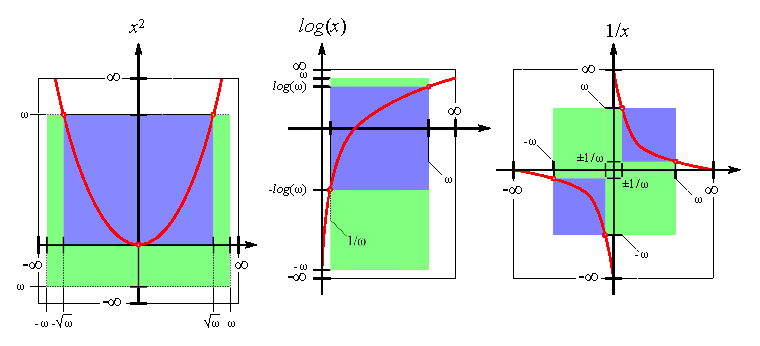
\includegraphics{Images/ExampleDomains.eps}
  \caption[Refined Domains of Primitive Functions]
          {Refined Domains of Primitive Functions}
  \label{fig:ExampleDomains}
\end{figure}

For the purpose of plotting an other analysis such as computing $P(Z < k)$ for $Z = f(X)$ a composite $f$ must be transformed into a piecewise monotonic $f$. The transformation process is referred to as \emph{refinment}. Function refinment serves two purposes. The first is to ensure that the numerical considerations are respected such that the associated function evaluates to a representable floating point value for every element of the domain. The second purpose is to ensure monotonicity within each domain interval.

\begin{figure}
  \centering
  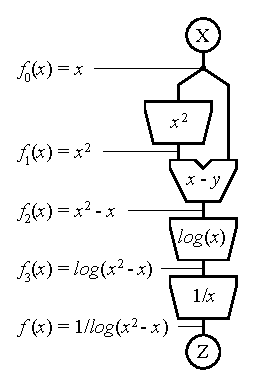
\includegraphics{Images/invlogX2minusXflow.eps}
  \caption[Parse Tree of $Z = 1/log(X^2 - X)$]
          {Parse Tree of $Z = 1/log(X^2 - X)$}
  \label{fig:invlogX2minusXflow}
\end{figure}

The refinment for several primitive functions is depicted in figure \ref{fig:ExampleDomains}  As a guiding example of the refinment process suppose that
\begin{align*}
Z = f(X) = \frac{1}{log(X^2 - X)}
\end{align*}
where
\begin{align*}
X \sim Normal(0,1) \text{ and } \mathcal{D}(X) = (-10,10)
\end{align*}
The parse tree of $f$ is a composition of primitive functions, composite function and arithmetic operator components is shown in figure \ref{fig:invlogX2minusXflow}. Transforming the composite $f$ into the piecewise monotonic $f$ is a sequention process that begins at the input $X$. Several composite function components are identified in figure \ref{fig:invlogX2minusXflow} including the indentity function $f_0(x) = x$. 

\begin{figure}
  \centering
  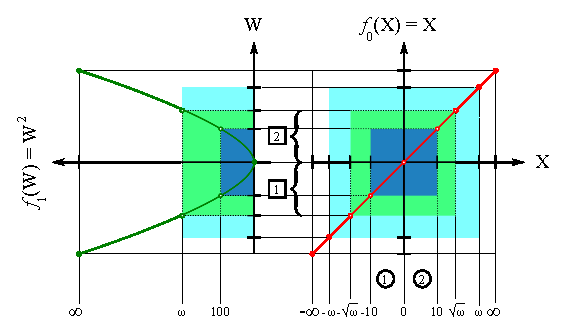
\includegraphics{Images/X.eps}
  \caption[Refinement $f_0(X)$ by $f_1(X)$]
          {Refinement $f_0(X)$ by $f_1(X)$}
  \label{fig:X}
\end{figure}

To begin, note that the domain of $X$ is the interval $(-10,10)$ which is assigned to be the domain of $f_0$. The next step is to consider the effect of $f_0$ of the adjacent node $x^2$ and the $y$-input of the operation $x-y$. Assume that $f_1(x)$ is refined in isolation of the containing $f(x)$ so that its initial definition is given in equation \ref{equation:x2}. The refinment process is to take the range of $f_0$, $(-10,10)$, and intersect it with the domain of $f_1$ into range components $\{(-10,0), (0,10)\}$ and find the pre-image under $f_0$ which is also $\{(-10,0), (0,10)\}$. This process is shown in figure \ref{fig:X} where \squared{1} = $(-\sqrt{\omega}, 0)$, \squared{2} = $(0, \sqrt{\omega})$, \circled{1} = $(-10,0)$, \circled{2} = $(0,10)$. 

In isolation the operation $x-y$ accepts any input in $(-\omega, \omega)$ so no further refinement is needed at this stage. Similarly no further refinement of $f_2$ is imposed by $x-y$. The domain of $f_2$ is then the set \{\circled{1}, \circled{2}\} in figure \ref{fig:X}.


\begin{figure}
  \centering
  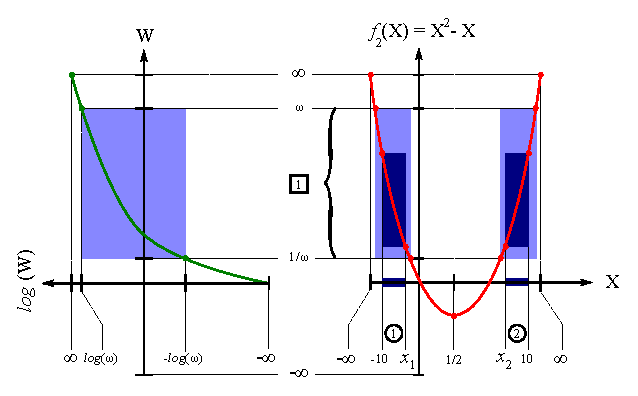
\includegraphics{Images/X2minusX.eps}
  \caption[Domain of $f_2(X)$]
          {Domain of $f_2(X)$}
  \label{fig:X2minusX}
\end{figure}

The domain of $f_2$ in the parse tree \ref{fig:invlogX2minusXflow} is refined by the domain of the primitive $log(x)$. Because $f_2$ involves a $2\times1$-dimensional transform, namely subtraction, and since the two operands are maximally entangled, the domain is less clearly defined and must be identified numerically. In general any value can be achieved by the transform $x-y$. Referring to the figure \ref{fig:X2minusX} the domain of $log(x)$ is \squared{1} = $(1/\omega, \omega)$. The domain of $f_2(X)$ is notated as before,
\begin{align*}
\mathcal{D}(f_2) &= \mathcal{D}(f_1) \cap f_2^{-1}(\mathcal{D}(log))\\
                    &= (-10,10) \cap \left((-\sqrt{\omega}, x_1) 
                                            \cup (x_4, \sqrt{\omega})\right)\\
                    &= (-10, x_1)  \cup (x_2, 10)
\end{align*}
where
\begin{align*}
x_1 = min \left\{ -f_2^{-1}(1/\omega),  -\frac{1}{\omega} \right\} && 
x_2 = max \left\{ +f_2^{-1}(1/\omega), 1+\frac{1}{\omega} \right\}
\end{align*}
Numerical considerations dictate that since $f_2^{-1}(1/\omega) < 1/\omega$ the nearest $x$-value within each domain interval must be found. At this stage the function $f_2$ is refined by $log(x)$ and piecewise defined as
\begin{align*}
f_2(x) = \begin{cases} x^2 - x \text{ if } x \in (-10, -\frac{1}{\omega})\\
                       x^2 - x \text{ if } x \in (1+\frac{1}{\omega}, 10)
         \end{cases}
\end{align*}

\begin{figure}
  \centering
  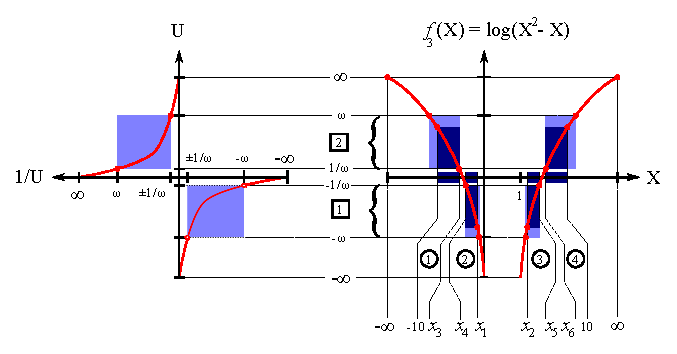
\includegraphics{Images/logX2minusX.eps}
  \caption[Domain of $f_3(X)$]
          {Domain of $f_3(X)$}
  \label{fig:logX2minusX}
\end{figure}

The last step of domain refinement in this example is shown in figure \ref{fig:logX2minusX}. Recall from \ref{fig:ExampleDomains} that the numerical domain of $1/x$ requires a small exclusion interval $C = (-1/\omega, 1/\omega)$. In isolation the primitive reciprocal function is defined on the piecewise domain $\{(-\omega, -1/\omega), (1/\omega, \omega)\}$. In figure \ref{fig:logX2minusX} the domains are \squared{1} and \squared{2} respectively. The pre-images under $f_3$ are then intersected with the domain of refined $f_2$ yielding the refined domain of $f_3$ as
\begin{align*}
\mathcal{D}(f_3) &= \mathcal{D}(f_1(X)) \cap f_3^{-1}(\{(-\omega, -1/\omega), (1/\omega, \omega)\}) \\
                    &= (-10, x_3) \cup (x_4, x_1) \cup (x_2, x_5) \cup (x_6, 10)
\end{align*}
In figure \ref{fig:logX2minusX} the refined domain of $f_3$ is shown as \circled{1}, $\dots$, \circled{4}. Notice that the intervals $(x_3,x_4)$ and $(x_5, x_6)$ were excluded from the the refined domain of $f_2$ and that they are very small and thus likely of negligible probability.


\begin{figure}
  \centering
  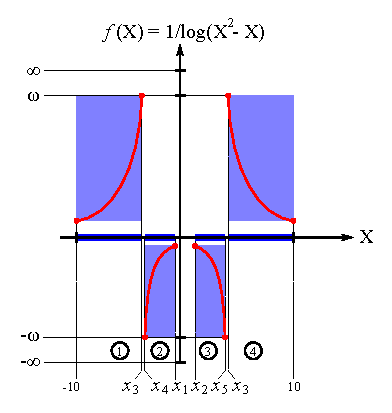
\includegraphics{Images/invlogX2minusX.eps}
  \caption[$Z = f(X)$ with Domain]
          {$Z = f(X)$ with Domain}
  \label{fig:invlogX2minusX}
\end{figure}

Notice that since $f$ does not feed into any other function elements in the example parse tree \ref{fig:invlogX2minusXflow} requires no further refinement. The final function of $f(X)$ is shown in figure \ref{fig:invlogX2minusX} with identified domain \{ \circled{1}, \circled{2}, \circled{3}, \circled{4} \}. 

\subsubsection{Combining Monotonic Functions of Random Variables}

The previous example revealed some important issues in computing functions of random variables. Breaking a function into non-overlapping monotonic fragments begs the question of how to locate interval endpoints. Domain refinement by intersection brought some numerical considerations when values became too small to represent as floating point values. The composition of two bijective functions is a bijective function, but the the same cannot be said for the sum or project of two bijections. The issue of refining a function that is the sum or product of bijections is addressed in this sub-section.

\begin{figure}
  \centering
  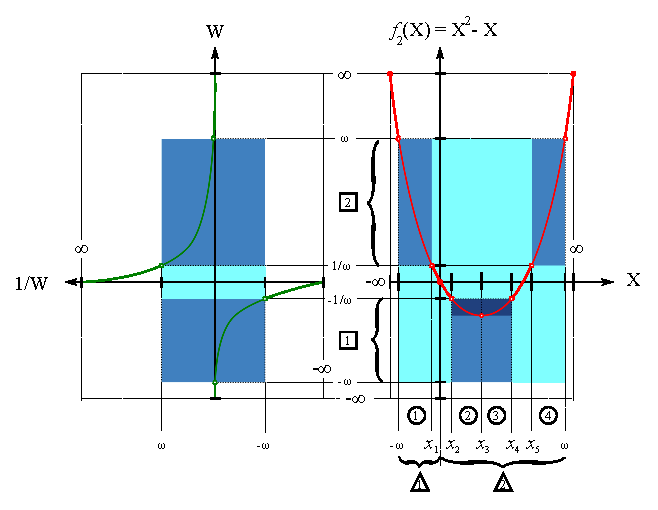
\includegraphics{Images/invX2minusX.eps}
  \caption[Refining $\frac{1}{x^2-x}$]
          {Refining $\frac{1}{x^2-x}$}
  \label{fig:invX2minusX}
\end{figure}

Consider the example,
\begin{align*}
f(x) = \frac{1}{x^2 - x}
\end{align*}
Since $f(x)$ contains $x^2$ the initial domain set is $\{(-\omega,0), (0,\omega)\}$ represented in figure \ref{fig:invX2minusX} by \triangled{1} and \triangled{2} respectively. Recalling the fundamental domain set of $1/x$ from figure \ref{fig:ExampleDomains} as $\{(-\omega, -1/\omega), (1/\omega, \omega)\}$ as \squared{1} and \squared{2} respectively.

Continuing with figure \ref{fig:invX2minusX}, the refined domain element \circled{1} is found by intersecting the pre-image of \squared{2} under $f$ given domain element \triangled{1}. Finding the refined domain element \circled{4} seems just a straightforward; the pre-image under $f$ given domain \triangled{2} intersected with \triangled{2}, but only because $f$ happened to be monotonic in \circled{4}. Notice that $f$ over domain element \triangled{2} is not monotonic. What is required is the intermediate step of refining each original domain element (\triangled{1} and \triangled{2} in this example) so that $f$ is monotonic over each domain element before further refining $f$ against $1/x$.

%%%%%%%%%%%%%%%%%%%%%%%%%%%%%%%%%%%%%%%%%%%%%%%%%%%%%%%%%%%%%%%%%%%%%%%%%%%%%%%%%%%%%%%%%%%


%%%%%%%%%%%%%%%%%%%%%%%%%%%%%%%%%%%%%%%%%%%%%%%%%%%%%%%%%%%%%%%%%%%%%%%%%%%%%%%%%%%%%%%%%%

\appendix
\chapter{Exhaustive Bounded Root Finding Method}
This section follows the \emph{EveryRoot} method developed by Robert C. Tausworthe \cite{tausworthe09} under contract with Raytheon, Inc.

Given an objective function $f$ defined on a normalized \emph{investigation} interval, $[0,1]$, the EveryRoot method finds nearly every root by exhaustive investigation. The EveryRoot method amalgamates several well-known root finding methods. By convention assume that $f_0 = f(0)$, etc.

\subsection{Specific Assumptions}
\begin{enumerate}
\item The objective function is presumed continuous on the investigation interval.
\item Given root $r$ it is presumed no other roots exist within interval $[r-xGuard, r+xGuard]$ for a prespecified tolerance value, $xGuard$.
\item A value $r$ is deemed to be a root if $|f(r)| \le \epsilon f$ for prespecified tolerance value $\epsilon f$ and $|f(r \pm xGuard)| > \epsilon f$.
\item If successive root estimates $r_i$ and $r_{i+1}$ differ by less than prespecified tolerance value $\epsilon r$ then $r_i$ is deemed to be a root of $f$.
\item If an interpolating polynomial $L$ of $f$ differs from the objective function at prespecified points within the interval by less than prespecified tolerance $\epsilon L$ then $L$ is deemed a \emph{reliable} facsimile of $f$.
\end{enumerate}

\subsection{Method Outline}
The general approach of the EveryRoot method is to recursively break the investigation interval $[0,1]$ into subintervals ultimately creating a partition where every subinterval contains exactly one or no roots. 

For any subinterval either none, one or both of the endpoints. If an endpoint is a root $r$ then it is centered in a \emph{guard} interval, $[r - xGuard, r+xGuard] \cap [0,1]$ where $r \in \{0,1\}$ and $[0,1]-([r - xGuard, r+xGuard] \cap [0,1])$ becomes the new investigation subinterval. 

Given the endpoints of $[0,1]$ are not roots, if $f_0f_1 < 0$ then at least one root exists in interval $(0,1)$. To find one of the possible roots in $(0,1)$ a \emph{bracketing} method such as Brent's Method \cite{brent73} or the much more recent Improved Brent's Method \cite{zhang11} is used. The internal root $r$ is found and guarded. The two flanking subintervals $[0,r-xGuard]$ and $[r+xGuard,1]$ are then investigated.

If $f_0f_1 > 0$ then the objective function $f$ is fit using an \emph{optimized} cubic Lagrange interpolation polynomial $L$. The optimization comes in the form of two specific function evaluation points within the investigation interval plus the two endpoints. The interpolation method is detailed below. The polynomial $L$ is deemed reliable upon evaluating it at three specific points within the interval where $L$ is most likely to differ from $f$ and finding that the relative error in all three cases is within $\epsilon L$ tolerance. If $L$ is un-reliable then the investigation interval is bisected into two subintervals. %i,e, we punt.

Suppose $L$ is a reliable facsimile of $f$ and $f_0f_1 > 0$. If $L$ has an extrema $e$ such that $f_0L_e < 0$, i.e. on the other side of zero from $f_0$ and $f_1$, and subsequently $f_0f_e < 0$ then the investigation interval is subdivided into $[0,e]$ and $[e,1]$ so that a bracketing method may be employed. If $L_e$ is \emph{relatively close} to zero then a \emph{root polishing} method such as Newton-Raphson or Halley's method maybe employed beginning at some other point in the interval. The method author suggests that if an extrema differs from zero with relative error less than a factor of three (3) of the fit tolerance $\epsilon L$ then $L_e$ is relatively close to zero. If there is no extrema of $L$ within the interval or none of the extrema are relatively close to zero then the interval is deemed to contain any roots.

\subsection{The \emph{EveryRoot} Method}
\todo{Write the algorithm, find test cases, then write this subsection.}

\subsection{Optimized Cubic Lagrange Interpolation}

Given an objective function $f$ over a normalized interval $[0,1]$ two internal points $0 < a < b < 1$ are chosen for fitting a cubic polynomial $L$,
\begin{align*}
L(x) = \alpha_0 + \alpha_1x + \alpha_2x^2 + \alpha_3x^3
\end{align*}
The corresponding four function evaluations are formed into the vector $\mathbf{f}$ where
\begin{align*}
\mathbf{f} = (f_0, f_a, f_b, f_1)^T
\end{align*}
Evaluating $L(x)$ at points $\{0,a,b,1\}$ and requiring $L(x)$ to equal $f(x)$ at those points yields the following linear relationship,
\begin{align*}
\begin{pmatrix}f_0\\f_a\\f_b\\f_1\end{pmatrix} = 
\begin{pmatrix}1&0&0&0\\1&a&a^2&a^3\\1&b&b^2&b^3\\1&1&1&1\end{pmatrix}
\begin{pmatrix}\alpha_0\\\alpha_1\\\alpha_2\\\alpha_3\end{pmatrix}
\end{align*}
The polynomial coefficients are found by inverting the matrix in the above equation,
\begin{align*}
\begin{pmatrix}\alpha_0\\\alpha_1\\\alpha_2\\\alpha_3\end{pmatrix} =
\frac{1}{D}
\begin{pmatrix}D&0&0&0\\
-(D+d)&b&-a&D\\
2d&-(b+1)&a+1&-d\\
-d&1&-1&d
\end{pmatrix}
\begin{pmatrix}f_0\\f_a\\f_b\\f_1\end{pmatrix}
\end{align*}
where $d = b-a,\; D = abd$ and it is assumed for symmetry that $b = 1 - a$.

%% Check the matrix in Python
\begin{comment}
def f(x): return (x-.1)*(x+1)*(x-2)    ## x^3 - 1.1x^2 -1.9x + 0.2
a = 1/3.; b = 1-a; d = b-a; D = a*b*d
f0 = f(0); fa = f(a); fb = f(b); f1 = f(1)
a0 = f0
a1 = 1/D*(-(D+d)*f0+b*fa-a*fb+D*f1)
a2 = 1/D*(2*d*f0-(b+1)*fa+(a+1)*fb-d*f1)
a3 = 1/D*(-d*f0+fa-fb+d*f1)
\end{comment}

\begin{figure}
  \centering
  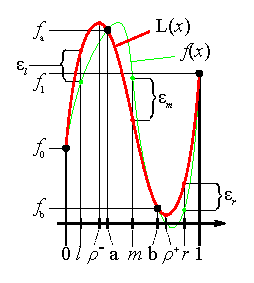
\includegraphics{Images/CubicLagrange.eps}
  \caption[Example Cubic Lagrange Interpolation]
          {Example Cubic Lagrange Interpolation}
  \label{fig:CubicLagrange}
\end{figure}

Figure \ref{fig:CubicLagrange} depicts an example interpolation with many of the elements discussed in this section present.

%% See ./library/InterpolationError.pdf
%% Available from: http://www.math.montana.edu/~davis/Classes/MA442/Sp07/Notes/InterpError.pdf
As may be found in any elementary calculus text the error of an $n^{th}$-order polynomial interpolation of $f(x)$ is given by
\begin{align}
L(x) - f(x) &= -\frac{f^{(n+1)}(c)}{(n+1)!}\prod_{i=0}^n(x - x_i)\\
\label{eq:TaylorError}
            &= \frac{f^{(4)}(c)}{4!}\;x(1-x)(x^2-x+a-a^2)
\end{align}
where $n=3$, $x_i \in \{0,a,1-a,1\}$ and for some $c \in (0,1)$. The largest errors occur at the extrema of the fourth-order polynomial $E(x) = x(1-x)(x^2-x+a-a^2)$ in the error expression. The extrema points are called \emph{ridge-error} points. Solving $E(x)$ for the ridge-error points,
\begin{align*}
\frac{d}{dx}E(x) = 0 \implies 
x = \left\{\frac{1}{2}\left(1\pm\sqrt{2a^2-2a+1}\right), \frac{1}{2}\right\}
\end{align*}
Evaluating $E(x)$ at each ridge-error point yields the unique extrema,
\begin{align*}
\left\{\frac{1}{4}a^2(1-a)^2, -\left(\frac{1-2a}{4}\right)^2\right\}
\end{align*}
Equating the absolute value of the two ridge-point extrema yields the following candidates for $a$,
\begin{align*}
2a(1-a) \equiv 1-2a \implies a = 1 \pm \frac{1}{\sqrt{2}}
\end{align*}
Since $a$ is required to lie in the interval $(0,\frac{1}{2})$ so that $0 < a < b < 1$, the ridge-point values are equated in absolute value by the choice
\begin{align}
a = 1-\frac{1}{\sqrt{2}} \approx 0.29289322
\label{eq:LagrangeInterpolationPoint}
\end{align}
Given this choice of $a$ the ridge-error points are,
\begin{align*}
l &= \frac{1}{2}\left(1-\sqrt{2a^2-2a+1}\right) = \frac{1}{2}\left(1 - \sqrt{2-\sqrt{2}}\right) \approx 0.117317\\
m &= \frac{1}{2}\\
r &= \frac{1}{2}\left(1+\sqrt{2a^2-2a+1}\right) = \frac{1}{2}\left(1 + \sqrt{2-\sqrt{2}}\right) \approx 0.882683
\end{align*}
and the $L(x)$ coefficients are found to be,
\begin{align}
\begin{pmatrix}\alpha_0\\\alpha_1\\\alpha_2\\\alpha_3\end{pmatrix} =
\begin{pmatrix}1&0&0&0\\
-(3+2\sqrt{2})&4+3\sqrt{2}&-(2+\sqrt{2})&1\\
4+4\sqrt{2}&-(10+7\sqrt{2})&8+5\sqrt{2}&-(2+2\sqrt{2})\\
-(2+2\sqrt{2})&6+4\sqrt{2}&-(6+4\sqrt{2})&2+2\sqrt{2}
\end{pmatrix}
\begin{pmatrix}f_0\\f_a\\f_b\\f_1\end{pmatrix}
\label{eq:LagrangeCoefficients}
\end{align}
%% Check the matrix in Python
\begin{comment}
def f(x): return (x-.1)*(x+1)*(x-2)    ## x^3 - 1.1x^2 -1.9x + 0.2

sqrt2 = 1.4142135623730950488016887242096980785696718753769480
a = 0.2928932188134524755991556378951509607151640623115259  ## 1-1/sqrt(2)
b = 1-a;
f0 = f(0); fa = f(a); fb = f(b); f1 = f(1)
a0 =                f0
a1 = -(3+2*sqrt2) * f0 + (4 +3*sqrt2) * fa - (2+  sqrt2) * fb +               f1
a2 =  (4+4*sqrt2) * f0 - (10+7*sqrt2) * fa + (8+5*sqrt2) * fb - (2+2*sqrt2) * f1
a3 = -(2+2*sqrt2) * f0 + (6 +4*sqrt2) * fa - (6+4*sqrt2) * fb + (2+2*sqrt2) * f1
\end{comment}
Let $A_{opt}$ be the matrix in the above equation. Noticing that
\begin{align*}
L(x) = (1,x,x^2,x^3)\;\begin{pmatrix}\alpha_0\\\alpha_1\\\alpha_2\\\alpha_3\end{pmatrix} = (1,x,x^2,x^3)\;A_{opt}\;\mathbf{f}
\end{align*}
it is possible to precompute \emph{ridge-error vectors}, $v_l, v_m, v_r$ corresponding to the ridge-error values $l, m, r$ found above for the sake of computational efficiency. Let
\begin{align*}
\mathbf{v}_k = (1,x_k,x_k^2,x_k^3)\;A_{opt} && \text{ for } && k \in \{l, m, r\}
\end{align*}
The ridge-error vectors are then,
\begin{align}
\mathbf{v}_l &= \frac{1}{4}\left(1+\sqrt{2-\sqrt{2}}, 1+\sqrt{2+\sqrt{2}}, 1-\sqrt{2+\sqrt{2}}, 1-\sqrt{2-\sqrt{2}}\right)^T\\
\mathbf{v}_m &= \frac{1}{4}\left(1-\sqrt{2}, 1+\sqrt{2}, 1+\sqrt{2}, 1-\sqrt{2}\right)^T\\
\mathbf{v}_r &= \frac{1}{4}\left(1-\sqrt{2-\sqrt{2}}, 1-\sqrt{2+\sqrt{2}},1+\sqrt{2+\sqrt{2}}, 1+\sqrt{2-\sqrt{2}}\right)^T
\label{eq:RidgeErrorVectors}
\end{align}
%% For Wolfram|Alpha
\begin{comment}
evaluate 1-x*(3+2*sqrt(2))+x^2*(4+4*sqrt(2)) -x^3*(2+2*sqrt(2)) where x = 1/2*(1-sqrt(2-sqrt(2)))
evaluate 0+x*(4+3*sqrt(2))-x^2*(10+7*sqrt(2))+x^3*(6+4*sqrt(2)) where x = 1/2*(1-sqrt(2-sqrt(2)))
evaluate 0-x*(2+sqrt(2))  +x^2*(8+5*sqrt(2)) -x^3*(6+4*sqrt(2)) where x = 1/2*(1-sqrt(2-sqrt(2)))
evaluate 0+x              -x^2*(2+2*sqrt(2)) +x^3(2+2*sqrt(2))  where x = 1/2*(1-sqrt(2-sqrt(2)))

simplify evaluate 1-x*(3+2*sqrt(2))+x^2*(4+4*sqrt(2)) -x^3*(2+2*sqrt(2)) where x = 1/2
simplify evaluate 0+x*(4+3*sqrt(2))-x^2*(10+7*sqrt(2))+x^3*(6+4*sqrt(2)) where x = 1/2
simplify evaluate 0-x*(2+sqrt(2))  +x^2*(8+5*sqrt(2)) -x^3*(6+4*sqrt(2)) where x = 1/2
simplify evaluate 0+x              -x^2*(2+2*sqrt(2)) +x^3(2+2*sqrt(2))  where x = 1/2

evaluate 1-x*(3+2*sqrt(2))+x^2*(4+4*sqrt(2)) -x^3*(2+2*sqrt(2)) where x = 1/2*(1+sqrt(2-sqrt(2)))
evaluate 0+x*(4+3*sqrt(2))-x^2*(10+7*sqrt(2))+x^3*(6+4*sqrt(2)) where x = 1/2*(1+sqrt(2-sqrt(2)))
evaluate 0-x*(2+sqrt(2))  +x^2*(8+5*sqrt(2)) -x^3*(6+4*sqrt(2)) where x = 1/2*(1+sqrt(2-sqrt(2)))
evaluate 0+x              -x^2*(2+2*sqrt(2)) +x^3(2+2*sqrt(2))  where x = 1/2*(1+sqrt(2-sqrt(2)))
\end{comment}
The ridge-error points and vectors are then used to compute the following set of interpolation errors,
\begin{align}
\epsilon_l &= |f(l) - \mathbf{v}_l^T \mathbf{f}\,|\\
\epsilon_m &= |f(m) - \mathbf{v}_m^T \mathbf{f}\,|\\
\epsilon_r &= |f(r) - \mathbf{v}_r^T \mathbf{f}\,|
\label{eq:RidgeErrorValues}
\end{align}
The \emph{EveryRoot} method uses the above interpolation errors to determine if $L(x)$ is a reliable facsimile to $f(x)$ over the normalized interval $[0,1]$. If $L(x)$ is deemed reliable the \emph{EveryRoot} method requires the extrema points of $L(x)$. These are found by solving the quadratic $L'(x) = 0$ and accepting only real roots, that is,
\begin{align*}
L'(x) &= 3\alpha_3\,x^2 + 2\alpha_2\,x + \alpha_1  = 0\\
\rho &=  -\frac{\alpha_2}{3\alpha_3} \pm \sqrt{\left(\frac{\alpha_2}{3\alpha_3}\right)^2-\frac{\alpha_1}{3\alpha_3}}
\end{align*}
The curvature of $L(x)$ is given by its second derivative,
\begin{align*}
L''(x) = 6\alpha_3\,x + 2\alpha_2
\end{align*}
When $L''(x)$ is evaluated at the extrema, if any, then the \emph{EveryRoot} method can decide if the extrema is near zero and warrents further investigation. Notice, for example, that in figure \ref{fig:CubicLagrange} the objective function $f(x)$ crosses zero even though $L(x)$ does not. The example in the figure has grossly exaggerated error values for $\{\epsilon_l, \epsilon_m, \epsilon_r\}$ and $L(x)$ would certainly be rejected by the \emph{EveryRoot} method as un-reliable. An interesting modification to the \emph{EveryRoot} method presents itself in the case of a reliability rejection; subdivide the interval into three parts, not two, namely $\{(0,a),(a,b),(b,1)\}$. The rationale for this modification is that each of the endpoints has already been evaluated so that $\{f_0, f_a, f_b, f_1\}$ are already in hand.

Notice further from the example depicted in figure \ref{fig:CubicLagrange} that because $L(x)$ is concave at the upper root, $\rho^+$, it seems a good place to initialize a root polishing method. In the figure it appears that a root is already found. This is accidental, but makes the point that even a reliable $L(x)$ should not be taken as a duplicate of the objective $f(x)$.

A rule to consider as a modification to the \emph{EveryRoot} method is if
\begin{align*}
|L(\rho)| < max\{\epsilon_l, \epsilon_m, \epsilon_r\}
\end{align*}
then root polishing should be initiated. A root polisher such as Halley's method, which approximates $f(x)$ with a parabola may best be initiated at the relevant $\rho$ and to bound it by the nearest known neighbors. In the figure the relevant extrema is $\rho^+$ and the bounding interval is $(b,r)$.

\subsubsection{Building the Interpolation Subroutine}

The \emph{EveryRoot} algorithm enters the Lagrange interpolation subroutine when $f_0f_1>0$, that is, the end points are on the same side of zero. The evaluations of $f_0$ and $f_1$ are assumed. The Lagrange interpolation subroutine must evaluate $f(x_a) = f_a$ and $f(x_b) = f_b$ to create the $\mathbf{\alpha}$ polynomial coefficients. Suppose $f_a$ is such that $f_0f_a < 0$, that is, on the other side of zero, then the two subintervals described by the partition $[0,a,1]$, are sent back to the \emph{EveryRoot} method where each is marked as known to contain at least one root.

Continuing with the interpolation subroutine, three more function evaluations at the ridge-error points must be made, namely, $\{f_l, f_m, f_r\}$. The total number of new function evaluations so far is five. If any of the ridge-error evaluations result in a zero crossing the appropriate partition of the investigation interval is sent back to the \emph{EveryRoot} method and each maked as known to contain at least one root. Suppose, for example, only $f_l$ crosses zero such that $f_0f_l < 0$ then the sub-partitition $[0,l,a]$ is sent back with each containing a root and the remaining $[a,1]$ is resent to the interpolation subroutine as an investigation interval since $f_af_1>0$.

At this point it is decided whether the interpolation is reliable. If not, there are five new interval endpoints that cannot be recycled so these become natural investigation subintervals, that is, the initial (normalized) interval is partitioned into six subintervals, $[0,l, a, m, b, r, 1]$ and each is re-fed in turn into the interpolation subroutine.

If the interpolation is deemed reliable then extrema are calculated. Either the extrema are real or not and if real inside the interval or not. If there is no extrema within the interval of positive curvature when $f_0 > 0$ and negative if $f_0 < 0$, in other words, close to zero, then the entire interval $[0,1]$ is marked as containing no roots and the subroutine ends.

If there is an extrema $\rho$ of appropriate curvature then a final function evaluation is made at $f_{\rho} = f(\rho)$. If $f_0f_{\rho}<0$ then the partition $[0,\rho,1]$ is sent back each known to contain a root otherwise the two nearest neighbor points are chosen and the roots of the derivative of the objective $f$ are found. For example in figure \ref{fig:CubicLagrange}, $\rho^+$  is the suggested minima. The nearest neighbors are $\{b, r\}$ and the true minima of $f$ could be left or right of $\rho^+$. 

Suppose the interval $[b,r]$ is suspected of containing the minima. If the endpoints are such that $f'(b) < 0$ and $f'(r)>0$ then a root bounding method applied to $f'$ over $[b,r]$ is used to find $\hat{\rho}$, the true minima of $f$. Otherwise the interpolation subroutine is re-entered over interval $[b,r]$ and the flanking intervals $\{[0,b]$, $[r,1]\}$ are marked as not containing roots. If $\hat{\rho}$ exists and $f_0f(\hat{r})>0$ the interval is declared to no contain a root else the intervals are $\{[b,\hat{\rho}], [\hat{\rho},r]\}$ each sent to the bounded root method since each contains a root. The possibility that $f(\hat{\rho}) \approx 0$ is considered and if true a single root is returned at $\hat{\rho}$.


%\chapter{Root Polishing}
%INFORMAL DISCUSSION

Since RICO is able to compute derivatives symbolically the family of Householder methods are available. \todo{reference other than Wikipedia}
Halley's Method is used in RICO. The reason is that it seems to provide a good performance and does not suffer from the tendency of Newtons to shoot beyond the bounded interval when a relatively flat spot of the objective function is encountered.

A problem shared by Newton and Halley is that there are initial points from with they fail to locate existing roots. They are therefore unreliable in discrediting the presence of a root, but very fast in determining the presence of a root.

Suppose that Halley's Method were unleashed on a bounded interval first. The cost is the number of function evaluations and the computation of the first and second derivative and their evaluations. At this point I have no way to decide when Newton or Halley is more appropriate. They share a deficiency. The derivative computations are symbolic and therefore relatively fast. The function evaluations are based on symbolic description and potentially fast depending on complexity of the description. The problem is that we're not so much interested in roots as determining that intervals do not contain roots. Finding a root only allows us to surround it with a tiny guard interval and return to searching the two flanking intervals. We usually don't know how many roots there are so we can't just look for roots.

I think Halley could be good at the tail end of the interpolation subroutine. 

%\chapter{Basic Design}
%A RandomVariable object is a combination of a DiscreteRandomVariable and a ContinuousRandomVariable objects. The continuous case is the focus since it's more challenging. 

Furthermore the focus at this level is one dimensional functions of random variables. Such functions are built up of components such as addition or multiplication by a constant, exponential powers such as $X^2$ as well as sums, difference, products and quotients of functions of the same random variable. The function that will form a running example in this section is,

\begin{align*}
Z = \ln(X + X^2)
\end{align*}

This is more generally expressed as,

\begin{align*}
Z = h(f(X) * g(X))
\end{align*}

where $*$ represents any binary operator such as $+, -, \times, \text{and } \div$.

\subsection{One Dimensional Functions of a Continuous Random Variable}

The goal of representing a continuous random variable is for the purpose of plotting it's probability density function for the user. We suppose that plotting a probability density function involves providing a partition of the real line. The software must then provide accurate estimates of the probability between each adjacent pair of partition elements. In an abuse of notation we write the partition of the resulting $Z$ random variable to be plotted as,

\begin{align*}
Z \sim (z_1, ..., z_{n+1})
\end{align*}

Then for each $i \in 1..n$ we must compute $Pr(z_i < Z \le z_{i+1})$. If $Z$ were a function of two random variables $X$ and $Y$ then each partition endpoint $z_i$ corresponds to a iso-curve in $(X,Y)$-space. This is still the case, but the iso-curves are isolated points, or possibly intervals in the case of function degeneracy.

The partition elements of the partition of $Z$ are indexed by their left-hand endpoint index. There are $n$ such partition elements. For each the software must locate the pre-image and compute the probability of this subset of the domain of $X$. The advantage of knowing all the range intervals at once and in particular knowing they are non-overlapping.

The running example $Z = \ln(X + X^2)$ is represented by the tree \ref{fig:ln_x_plus_x2}

\begin{figure}
  \centering
  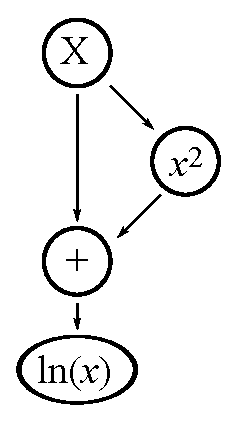
\includegraphics{Images/ln_x_plus_x2.eps}
  \caption[Tree of $Z = ln(X + X^2)$]
          {Tree of $Z = ln(X + X^2)$}
  \label{fig:ln_x_plus_x2}
\end{figure}


The basic algorithm to compute the pre-image of the $Z$ partition (itself a partition) is,

\begin{enumerate}
\item If any function block is of form $x^{-|p|}$ find and mark the pole in the $X$ domain.
\item Pick an initial $x$-value. The median may be the most convenient.
\item Ensure that each function block in the tree satisfies the domain requirements.
\item If domain requirements are not satisfied then find the extents of the domain violation.
\item For the working $x$-value find the extents of the current partition.
\item For each unidentified interval in the $X$ domain, goto step 2.
\end{enumerate}

The algorithm requires much explaining. The first step is the \emph{pole identification} step. There are no poles in the running example. If one of the blocks is of the form $x^{-2}$, for example, then we trim the tree before the reciprocal block and perform a root-finding step.

\subsubsection{Root Finding}

Given a function $f(X)$ we want to find all values $x \in X$ so that $f(x) = 0$. The general state of $X$ is that some or all poles are identified with some bounding interval and some or all domain violation regions are similarly marked with a bounding interval. If the root finding step is taking place in the context of initial pole identification then no regions will yet be indentified as the pre-image of the $Z$ partition since it's not yet specified.

Each unexplored region in $X$ must be explored for a possible. The bounded Halleys Algorithm is detailed below. It requires the computing of the first and second derivatives of $f(X)$ where we suppose,

\begin{align*}
g(X) = f(X)^{-|p|}
\end{align*}

A significant issue is finding the multiple roots, if any. A saving grace is that we work from the inside out. There should be no unidentified poles in $f(X)$. This means that if we chase a tail and we don't have a boundary in front of us we can safely mark the extents as explored. Using Halley's Method (bounded or unbounded) we always explore both directions from the initial $x$.

Another feature we might consider is the identification of polynomial expressions. Polynomial root-finding is a special case. Linear is even more special. 

%\section{Simplify}
A Rico object may represent a function whose operands are themselves Rico objects. A Rico Object then forms a \emph{parse tree}. The reference to \emph{parsing} stems from a tree of Rico objects being created in response to user interaction or user-provided algorithm. The possibility of algorithmic creation of parse trees drives the focus to expression simplification since algorithms may generate parse trees that involves tens or even tens of millions of terms.

As detailed elsewhere not all forms of algebraically equivalent expressions are equally easy to evaluate numerically. As an example consider $X + XY$ where $X$ and $Y$ are mutually independent random variables. The addition operation between $X$ and $XY$ is not simple since the operands are algebraically correlated. However, the equivalent expression, $X(1+Y)$ involves the addition and multiplication of mutually independent random variables. Independent combinations of random variables tend to be easier to implement numerically than correlated combinations since there is no correlation component.

Another reason for expending the design cost of creating a function that simplifies Rico parse trees is to reduce the evaluation work load. For example, an expression such as $(X+X^2)/X$ is better represented as the algebraically equivalent $1+X$. Similarly $log(exp(X))$ is better represented as $X$. While a user may not type such an expression as $log(exp(X))$, an algorithm may generate it or it may arise as an intermediate step in the simplification process itself.

Rather than attempting to define a \emph{simplification} metric for all admissible expressions, the goal of this section is to demonstrate that the process called \emph{simplification} within the Rico project reliably produces algebraically equivalent output expressions for any admissible input expression and tends to produce simpler equivalent expressions. 

The simplification algorithm is detailed below. It employs expression simplification heuristics that will also be detailed. A testing regimine will be detailed and the claim that the testing regimine will guarantee the claim of expression equivanence. 

\subsection{Simplification Overview}
When given an arithmetic expression in the form of a Rico object representing an expression parse tree the simplification algorithm will recursively call itself on any operand objects (also called \emph{child} objects) forming a \emph{depth-first} algorighm. This knowledge allows each step in the algorithm to assume that any operand objects are in \emph{simplest form}. The definition of \emph{simplest} in this context is itself recursive. The meaning of \emph{simplest} emerges within the simplification steps.

The simplification algorithm is comprised of several stages, the first is properly called the simplifying step. The purpose of this step is to remove all integer exponents (save $1$ and $-1$) from sums of objects, recover identity operations such as $exp(log(X)) \rightarrow X$ and $X/X \rightarrow 1$, generally convert any expression to the quotient of sums of products to the extend possible. 

Under certain circumstances division of polynomials may be attempted in secondary stages of simplification. A conditional last stage of simplification is factoring of common terms.

Another motivating example is,

\begin{align*}
\frac{(x+2)^2 +1}{x^2 + 4x + 5} \rightarrow 1
\end{align*}

The components to the simplification algorithm are described below with the lowest order first.

\subsection{Rico Objects}

Before expression simplification is attempted the admissible expressions must be detailed. For the most part Rico creates it's parse tree as numerical operations are encountered. If, for example, the user directs Rico to form the square root of a Rico object, the result is a square root object with the starting object as the sole operand. The process is similar for log, exp, subtraction, division, etc. The exceptions are addition, multiplication and exponentiation (or power).

There are three basic kinds of Rico objects to consider during simplification; NaN, numeric, and non-numeric where \emph{NaN} stands for not-a-number. A NaN Rico object arises to indicate a result is undefined such as 0/0, etc. A numeric Rico object is one of the allowed numeric types such as integers, floating point values and fractions (of integers). A non-numeric Rico object represents either a built-in random variable or a function of Rico objects whose result is not numeric and well defined (not NaN). 

It is convenient to use compact symbols to represent the three kinds of Rico objects,

\begin{align*}
\phi &\text{ is a NaN Rico object}\\
\nu  &\text{ is a numeric Rico object}\\
\rho &\text{ is a non-numeric Rico object}
\end{align*}

and capital letters such as $X$, near end of alphabet represent generic Rico objects.

\subsubsection{Simplify Negate}

The negation simplifier accepts one operand and obeys the following rules,

\begin{align*}
-\{\phi\}          &\rightarrow \phi\\
-\{\nu\}           &\rightarrow -\nu\\\
-\{\nu \times X\}  &\rightarrow \{-\nu\} \times X\\
-\{X\}             &\rightarrow \{-1\} \times X
\end{align*}

The $-\{\nu \times X\}$ rule allows number objects to absorb the negation operation. The last rule replaces the negation operation with the product of $X$ and $-1$, in the conventional number-first order.

\subsubsection{Rico Addition}

The Rico addition object accepts two or more operands. There are four cases for each operand, 

\begin{align*}
\{\phi, 0, \nu, \rho\}
\end{align*}

where it is understood that a rule that applies to zero is selected before a generic number $\nu$ and $X$ applies to any Rico object. Since the rules are applied in order the specific $\rho$ symbol tends not to appear. Rather, the generic $X$ (and subsequent generics) appear most often.

Several features are accommodated in the following rules,

\begin{enumerate}
\item Propagate $NaN$ values
\item Discard zeros
\item Perform numeric addition
\item Ensure number objects appear in first position in list of operands
\item Perform coefficient addition
\item Collapse cascaded addition operations
\end{enumerate}

These rules may be encoded as if there are only two operands as follows,

\begin{align*}
\phi + X                   &\rightarrow \phi\\
X + \phi                   &\rightarrow \phi\\
X + 0                      &\rightarrow X\\
0 + X                      &\rightarrow X\\
\nu_1 + \nu_2              &\rightarrow \{\nu_1+\nu_2\}\\
X + \nu                    &\rightarrow n + X\\
\nu_1 \times X + \nu_2 \times X  &\rightarrow \{\nu_1 + \nu_2\} \times X\\
X + (Y + Z)                &\rightarrow X + Y + Z\\
(X + Y) + Z                &\rightarrow X + Y + Z\\
X + Y                      &\rightarrow X + Y
\end{align*}

When there are more than two operands the behaviour is as if an accumulation of two-operand addition operations, i.e. $(X+Y+Z) = ((X+Y)+Z)$.

\subsubsection{Rico Multiplication}
Within Rico multiplication is handled in a similar manner to addition. Cascades products are flattened, zeros and NaN's dominate expressions and ones are filtered out. The rules are then,

\begin{align*}
NaN*Y             &\rightarrow NaN\\
X*NaN             &\rightarrow NaN\\
X*0               &\rightarrow 0\\
0*Y               &\rightarrow 0\\
X*1               &\rightarrow X\\
1*Y               &\rightarrow Y\\
(X*Y)*Z           &\rightarrow X*Y*Z\\
X*(Y*Z)           &\rightarrow X*Y*Z\\
(X*Y)*(Z*K)       &\rightarrow X*Y*Z*K
\end{align*}

As in the addition case the $NaN$ dominates the output of any function. Like the $NaN$ value, zero dominates the multiplication output. Note in particular that $NaN$ dominates zero. The next two rules involving one are the equivalent nullification as the zero is for addition. The last three rules detail the expression flattening of cascaded products. 

\subsubsection{Rico Power}

The Power function, $X^Y$, requires more care so it doesn't provide any automatic flattening of cascaded powers as addition and multiplication do provide. There are still the automatically applied rules for $NaN$, $0$ and $1$,

\begin{align*}
X^{NaN}                        &\rightarrow NaN\\
{NaN}^Y                       &\rightarrow NaN\\
{NaN}^{NaN}                    &\rightarrow NaN\\
(X1 + \dots +X3)^n            &\rightarrow X1^n + \dots + X3^n\\
(X1 \times \dots \times X3)^Y &\rightarrow X1^Y \times \dots \times X3^Y\\
(X^Y)^Z                       &\rightarrow X^{Y \times Z}\\
exp(X)^Y                      &\rightarrow exp(X \times Y)\\
{n1}^{n2}                      &\rightarrow n3\\
X^0                           &\rightarrow 1\\
X^1                           &\rightarrow X
\end{align*}

The ${n1}^{n2} \rightarrow n3$ rule is triggered when both operands are numeric values and the rule says to evaluate these two operands into a single numeric value, possibly $Nan$. The numeric power rule is detailed below.

The rule $(X1+X2+...+X3)^n \rightarrow X1^n + ... + A3^n$ assumes an integer exponent. The distributive law is them applied so that the result is a sum of powers. 

The rule $(X1 \times \dots \times X3)^Y \rightarrow X1^Y \times \dots \times X3^Y$ distributes powers over each product operand. This rule is in keeping with the overall strategy of exploring legal interactions bewteen operands. A later factoring step for exponents will recover the original form if possible.

The rule $X^0 \rightarrow 1$ presumes that $X$ is non-numeric. This is no guarantee that $X$ does not represent a random variable with non-zero probability concentrated at zero or either infinity. This rule will need to be revisited when discrete random variables are introduced. Doubtless this rule will be removed at that point.

\subsubsection{Rico Numeric Power}

The special case results of the power evaluation of two numeric values are detailed in table XXX.

\vspace{.1 in}
\begin{tabular}{|c|cccccl||}
\hline
$x^y$     & $0$   & $1$       & $+\infty$ & $-\infty$  & $NaN$ & $d2$\\
\hline \hline
$0$       & $NaN$ & $0$       & $0$       & $NaN$      & $NaN$ & $\{NaN, 0\}    \sim \{-,+\}$\\
$1$       & $1$   & $1$       & $NaN$     & $NaN$      & $NaN$ & $1$ \\
$+\infty$ & $NaN$ & $+\infty$ & $NaN$     & $NaN$      & $NaN$ & $\{0, +\infty\} \sim \{-,+\}$\\
$-\infty$ & $NaN$ & $NaN$     & $NaN$     & $NaN$      & $NaN$ & $\{0, -\infty\} \sim \{-,+\}$\\
$NaN$     & $NaN$ & $NaN$     & $NaN$     & $NaN$      & $NaN$ & $NaN$ \\
$d1$      & $1$   & $x$       & $sgn(d1) \infty$ & $0$ & $NaN$ & ${d1}^{d2}$ \\
\hline
\end{tabular}

The expression $\{0, -\infty\} \sim \{-,+\}$ in the last column means that $0$ is chosen if $d2 < 0$ else $-\infty$ is chosen. There is no possibility for $d2$ to be zero since that case is already addressed.

\subsubsection{Equality Test}

Several parts of the simplification algorithm rely on the ability to compare two objects for equality. Two Rico objects are \emph{equivalent} if they are of the same Rico type and if they have child objects (operands for functional objects) then, modulo order in the case of addition and multiplication, those child objects are also equivalent.

The following Rico objects (expressions) are then equivalent,

\begin{align*}
X+Y+3 &\equiv 3 + X + Y\\
X*5 &\equiv 5X
\end{align*}

but many algebraically equivalent expressions are not equivalent in the Rico sense. For example,

\begin{align*}
(X+2)^2 + 1 &\neq X^2 + 4X + 5
\end{align*}

Note especially that Basic random variables are a special type of Rico object. Basic random variables are issued a unique id code upon creation and two Basic random variables are distinguished by id code, not random variable type. For example if $X = Normal(2,3)$ and $Y = Normal(2,3)$, then $X \equiv Y$ iff $id(X) = id(Y)$. 

Rico Numbers are equivalent if they represent identical values. Floating point Numbers are equivalent if they are within a specific numerical tolerance to compensate for minor least significant bit differences. Fractions in Rico are easily compared by comparing their integer numerator and denominator since they are always represented in lowest form with the numerator carrying the signed value.

\subsection{Simplify Stage One}

Stage One of the simplify algorithm is depth-first. At each node Stage One of the simplify algorithm is called and upon return a transformation appropriate to the current object is called. If the current object is a function and therefore has child objects (operands) then they are assumed to have already been Stage One simplified.

The Stage One object simplifications are detailed by object type. Many simplifications build on each other. 

\subsubsection{Simplify Subtract}

The subtration function in Rico accepts exactly two operands. The Stage One simplification is to transform subtration to addition as follows,

\begin{align*}
A - B \rightarrow A + \{-1\}*B
\end{align*}

The end result is that a Stage One simplified expression contains no subtraction functions.

\subsubsection{Simplify Division}

Analagously to the subtraction function, the division function is transformed as,

\begin{align*}
A \div B \rightarrow A * B^{-1}
\end{align*}

\subsubsection{Simplify Square Root}

Building on the division function transformation there is replacement of the square root function,

\begin{align*}
\sqrt{A} \rightarrow A^{\frac{1}{2}}
\end{align*}

\subsubsection{Simplify Log}

The Stage One simplification huristic is to turn products of sums to sums of products. This extends to the following transformation rules,

\begin{align*}
log(exp(X)) &\rightarrow A\\
log(X^Y)    &\rightarrow Y*log(X)\\
log(X*Y*Z)  &\rightarrow log(X)+log(Y)+log(Z)
\end{align*}

In this way, multiplication within a function is exposed outside as addition. 

\subsubsection{Simplify Exp}

By similar reasoning to Stage One log simplification the exp rules are,

\begin{align*}
exp(log(X)) &\rightarrow A
exp(X+Y+Z)  &\rightarrow exp(X)*exp(Y)*exp(Z)
\end{align*}

In this way, addition within a function is exposed outside as multiplication. 

\subsubsection{Simplify Addition}

A Rico addition object may contain two or more operand objects. The hallmark transformation at this stage is,

\begin{align*}
3X + X \rightarrow 4X
\end{align*}

Notice that $3X$ is a multiplication object that contains a number object as an operand. It is assumed that the Stage One Multiply simplification has already occurred and that this multiplication object contains zero or one number object operands and furthermore if a number object is present it is the first operand in the list of operands. A further consideration is seen in the following transformation,

\begin{align*}
3XY + X + YX \rightarrow 4XY + X
\end{align*}

The number object ($3$) in the above expression is commonly referred to as the coefficient of the expression. This coefficient must be split from the three operand multiply object into a number object and a two operand multiply object. The latter is referred to as the \emph{base} object. Unique base objects is must be identified and the coefficients of any duplicated base objects are summed. Two related special cases are addressed as follows,

\begin{align*}
2XY + X + -2XY &\rightarrow X\\
2XY + -2XY     &\rightarrow 0
\end{align*}

\subsubsection{Simplify Multiplication}

Multiplication simplification returns $NaN$ if any openand is of type $NaN$. The distributive law is then applied, as needed, and the result is a sum of Stage One simplified products.

\begin{align*}
X \times NaN   &\rightarrow NaN \\
NaN \times Y   &\rightarrow NaN \\
NaN \times NaN &\rightarrow NaN\\
(X+Y) \times Z &\rightarrow XZ + YZ\\
X \times (Y+Z) &\rightarrow XY + XZ\\
X^Y \times X^Z &\rightarrow X^{Y+Z}\\
n1 \times n2  &\rightarrow n3\\
(X \times Y) \times (Y \times Z) &\rightarrow XY^2Z
\end{align*}

The last term applies to an operand that is itself a product of an arbitrary number of operands. For example,

\begin{align*}
(X \times 2 \times Y) \times (Y \times Z) &\rightarrow 2XY^2Z
\end{align*}

\subsection{Simplify Stage Two}

\todo{This needs to be fleshed out. First the StageOne Simplify needs to be completed.}

\subsubsection{Factoring}
The Factor tree operation is depth-first. It acts at addition nodes to factor out common nodes from sums of products of nodes. Two example transformations are,

\begin{align*}
AB + AC + D         &\rightarrow  A(B+C) + D\\
5A + 5^2AB + 5^3ABC &\rightarrow  5A(1 + 5B(1 + 5C))
\end{align*}

where the juxtaposition implies multiplication of the separate nodes $A, B, C$. The first transformation demonstrates that the $A$ node need not be common to all products. The second transformation comes from the concept of Net Present Value.

\todo{Define what happens to fractional powers}

The expression $AB + AC + BC$ may be factored as $A(B+C) + BC$ or $B(A+C) + AC$ demonstrating that factorization is not uniquely defined. The Factor tree operation is implemented using a \emph{sparse product matrix}. 

An example without non-unit exponential is first considered. Given the expression,

\begin{align*}
AB + AC + D
\end{align*}

A list of uniqe nodes is constructed; $\{A, B, C, D\}$. Using this list to define the columns referred to as a \emph{header}, a sparse matrix of powers is constructed where each row represents a product of header elements and the rows collectively represent the sum of products. The sparse product matrix for this example is then,

\begin{align*}
\begin{pmatrix}A & B & C & D\\1 & 1 & &\\1 & & 1 &\\& & & 1\end{pmatrix}
\end{align*}

The $A$ is most common element since it appears in more rows than any other header element it is chosen as the factored element. If another header element, say $B$ had been as common as $A$ then the powers of $A$ and $B$ would be summed and the greater chosen as the factored element. If a tie persist then the first of the tied element in the header list is chosen.

To factor out the $A$, the sparse matrix rows are partitioned into those including the $A$ element and not. Two new sparse product matrices are created. It is convenient that the headers of each are simple copies of the original header $\{A, B, C, D\}$. Since the matrices are sparse there is no computational cost beyond a possible header copy operation. The resulting expression may be written as,

\begin{align*}
  \begin{pmatrix}A & B & C & D\\
                 1 & 1 &   &  \\
                 1 &   & 1 &\end{pmatrix} 
+ \begin{pmatrix}A & B & C & D\\
                   &   &   & 1 \end{pmatrix}
\end{align*}

The $A$ expression is now formally factored out and for a reason that will be made clear below zeros are left in the $A$ column of the first matrix,

\begin{align*}
A \times\begin{pmatrix}A & B & C & D\\
                       0 & 1 &   &  \\
                       0 &   & 1 &\end{pmatrix} 
+       \begin{pmatrix}A & B & C & D\\
                       &   &   & 1 \end{pmatrix}
\end{align*}

The Factor operation recurses until no further factoring is possible as is the case in the example above for both sparse product matrices. The resulting expression is then,

\begin{align*}
A \times (B + C) + D
\end{align*}

To introduce further considerations a second example is warrented. Consider the expression,

\begin{align*}
5A + 5^2AB + 5^3ABC
\end{align*}

The corresponding sparse matrix is,

\begin{align*}
\begin{pmatrix}5 & A & B & C\\
               1 & 1 &   &  \\
               2 & 1 & 1 &  \\
               3 & 1 & 1 & 1\end{pmatrix}
\end{align*}

The $5$ and the $A$ are equally common and the tie is broken by the sum of powers which is $6$ for the $5$ node and only $3$ for the $A$ node. The $5$ is then factored, but instead of creating two sparse product matrices only one needs be created since the $5$ appears in all rows and the expression becomes,

\begin{align*}
5 \times \begin{pmatrix}5 & A & B & C\\
                        0 & 1 &   &  \\
                        1 & 1 & 1 &  \\
                        2 & 1 & 1 & 1\end{pmatrix}
\end{align*}

Since the $A$ is now most common it is factored and only one sparse product matrix results again,

\begin{align*}
5 \times A \times \begin{pmatrix}5 & A & B & C\\
                                 0 & 0 &   &  \\
                                 1 & 0 & 1 &  \\
                                 2 & 0 & 1 & 1\end{pmatrix}
\end{align*}

Now $5$ and $B$ are most common, but $5$ has more power. Now the reason for the zero's becomes clear because we must leave a one in the place of the first row,

\begin{align*}
5 \times A \times \Big(
\begin{pmatrix}5 & A & B & C\\
               0 & 0 &   &  \end{pmatrix}
+
\begin{pmatrix}5 & A & B & C\\
               1 & 0 & 1 &  \\
               2 & 0 & 1 & 1\end{pmatrix}
\Big)
\end{align*}

The zero row of the first matrix resolves to a one and the $5$ of the second matrix is factored,

\begin{align*}
5 \times A \times \Big(1 
+ 5 \times 
\begin{pmatrix}5 & A & B & C\\
               0 & 0 & 1 &  \\
               1 & 0 & 1 & 1\end{pmatrix}
\Big)
\end{align*}

Next the $B$ is factored and the matrices can be replaced by their equivalent expressions with juxtaposition in place of multiplication,

\begin{align*}
5A \Big(1 + 5B(1 + 5C)\Big)
\end{align*}




%\chapter{Correlated Operations}
%Given a random variable $A$ and two real-valued functions $f$ and $g$ such that $X = f(A)$ and $Y = g(A)$ let $Z = h(X,Y)$ where $h$ is some real-value function from $\mathbb{R}^2$. The function $h(x,y) = x+y$ is of particular interest.

Since $A$ may be a mixed random variable the development will by assuming $A$ is discrete, then continuous and finally a general mixed random variable. In all cases $X$ and $Y$ are, by design, 100\% correlated through $A$.

\subsection{Discrete Operations on Correlated Random Variables}

Suppose that,

\begin{align*}
A = ((a_1, a_2, ..., a_n), (p_1, p_2, ..., p_n))
\end{align*}

where $Pr[A = a_i] = p_i$ for any $i \in 1...n$, that is, $A$ is a discrete random variable. Consequently,

\begin{align*}
X = ((x_1, x_2, ..., x_n), (p_1, p_2, ..., p_n))\\
Y = ((y_1, y_2, ..., y_n), (p_1, p_2, ..., p_n))\\
\end{align*}

where $x_i = f(a_i)$ and $y_i = g(a_i)$  for each $i$. Notice that duplicate values of $x_i$ are possible. If it happens that $x_i < x_{i+1}$ for each $i \in 1...n-1$ then $X$ is said to be in \emph{proper form} and similarly for $A$ and $Y$. To emphasize that $X$ and $Y$ are derived in a pointwise order-preserving manner they may be written in \emph{synchronous} form,

\begin{align*}
X = (x_1, x_2, ..., x_n)\\
Y = (y_1, y_2, ..., y_n)
\end{align*}

where the probability values associated with each $x_i$ and $y_i$ are found in $A$. The joint probability distribution of $X$ and $Y$ is itself a random variable called $XY$. Stated in syncrhonous form,

\begin{align*}
XY = ((x_1, y_1), (x_2, y_2), ..., (x_n, y_n))
\end{align*}

A new random variable $Z = h(X,Y)$ is stated in synchronous form with respect to $A$ as,

\begin{align*}
Z &= (h(x_1, y_1), h(x_2, y_2), ..., h(x_n, y_n))
\end{align*}

To restate $Z$ in proper form requires two steps. The first is to remove duplicates form the range of $Z$,

\begin{align*}
\mathbf{R}(Z) = \{h(x_i, y_i)\}_{i \in 1..n}
\end{align*}

The second step is to find the probability associated with each element of the range of $Z$. Assuming the following proper form of $Z$ as,

\begin{align*}
Z = ((z_1, z_2, ..., z_m), (q_1, q_2, ..., q_m))
\end{align*}

where $m \le n$ then,

\begin{align*}
z_j &\in \mathbf{R}(Z) \text{, ordered ascending}\\
q_j &= \sum_{i | z_j = h(x_i, y_i)}p_i
\end{align*}

For example suppose,

\begin{align*}
A = ((a_1,a_2,a_3),(p_1,p_2,p_3))\\
X = (1,2,3)\\
Y = (1,3,2)
\end{align*}

The joint random variable $XY$ in synchronous form is,

\begin{align*}
XY = ((1,1), (2,3),(3,2))
\end{align*}

Suppose $Z = h(X,Y)$ where $h(x,y) = x+y$. Then $Z$ in synchronous form with respect to $A$ is,

\begin{align*}
Z = (2, 5, 5)
\end{align*}

To find the proper form of $Z$ the range is first determined,

\begin{align*}
\mathbf{R}(Z) = \{2,5\}
\end{align*}

the proper form of $Z$ is stated as,

\begin{align*}
Z = ((z_1, z_2), (q_1, q_2))
\end{align*}

where

\begin{align*}
q_1 &= p_1\\
q_2 &= p_2 + p_3
\end{align*}

since $Z = 5$ is the set $\{(x_2,y_2) = (2,3), (x_3, y_3) = (3,2)\}$. Notice that the process of finding $Z$ in proper form is that of integrating iso-value subsets of the joint $XY$ range, the domain of $Z$. 

\subsection{Continous Operations on Correlated Random Variables}

Suppose $A$ is a real-valued continous random variable. Let $P$ be the probability density function associate with $A$ and write $A \sim P$. The random variables $X = f(A)$ and $Y = g(A)$, in synchronous form, share this association with $A$, that is, $X ~ P$ and $Y ~ P$ for any real valued functions $f$ and $g$. The joint random variable $XY$ is also stated in synchronous form as $XY \sim P$. Finally, $Z = h(XY)$ for any real-valued function $h$ from $\mathbb{R}^2$ is also stated in synchronous form as $Z \sim P$. 

To form an interesting example consider that $X = f(A)$ and $Y = g(A)$ form a parametric curve in $XY$-space and that the probability density $P$ is distributed along this curve. If $Z = h(XY)$ such that $h(x,y) = x+y$ then iso-value contours in $XY$-space appear as parallel lines with slope $-1$. In the figure \ref{fig:XY_continous} the disjoint curves are the single parametric $(X,Y)$ curve and the dotted diagonal lines are the iso-value contours for addition of $X$ and $Y$. The probability density $P$ of $A$ would appear in the figure perpendicular to the $XY$ plane over the paremetric curve of $(X,Y$). From the figure it is apparent that $Pr(1 < Z < 5) = 1$. Notice that the iso-value contour labeled $5$ in the figure intersects the $XY$ curve at three places so that $Pr(Z = 4)$ is found as the sum of three probability density values in $P$. 

\begin{figure}
  \centering
  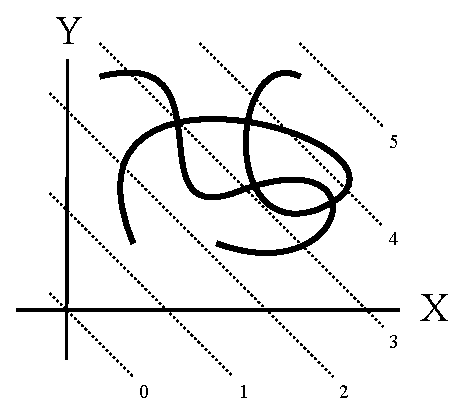
\includegraphics{Images/XY_continous.eps}
  \caption[Joint distribution of correlated Continuous $X$ and $Y$ in $XY$-space]
          {Distribution of Continuous $XY$}
  \label{fig:XY_continous}
\end{figure}

Stating the synchronous form of $Z$ with respect to $A$ is as simple as for $X$ and $Y$, that is, $Z \sim P$. Finding the proper form of $Z$ may be a more challenging problem. The procedure for computing a numerical approximation to the proper form of $Z$ is detailed in the dissertation \cite{fielden12}. Notice in particular that computing the proper form of a random variable may be avoided until and observation is required for reasons such as graphing or comparison to unrelated random variables and constant values.

\subsection{Mixed Discrete / Continuous Operations on Correlated Random Variables}

To prepare for the computation of operations on a pair of mixed discrete/continuous random variables dependent on a single common random variable, it is useful to develop the case where one operand is discrete and the other is continuous. This situation can only arise if $A$ is not a purely discrete random variable.

Suppose that $A$ is a continuous random variable such that $A \sim P$ as above. Suppose without loss of generality that $X$ is a discrete random variable and that $Y$ is a continuous random variable. A visual example of a possible joint random variable $XY$ appears in figure \ref{fig:XY_discrete_continuous}. Included in the figure are the iso-value contours used to compute $Z = h(XY)$ where $h(x,y) = x+y$ as the previous continous example. Notice that this case is not fundamentally different from the previous case where $X$ and $Y$ are both continous. In the figure $X$ has four unique values in its range labeled $x_1, x_2, x_3, x_4$. It is apparent from the figure that $Pr(1 < Z < 5) = 1$ and that $Z$ is a continuous random variable. The procedure for computing a numerical approximation to the proper form of $Z$ is detailed in the dissertation \cite{fielden12}. 

\begin{figure}
  \centering
  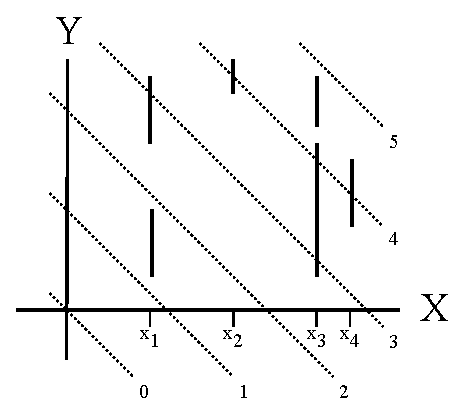
\includegraphics{Images/XY_discrete_continous.eps}
  \caption[Joint Distribution of Correlated Discrete $X$ and Continous $Y$ in $XY$-space]
          {Distribution of Discrete/Continous $XY$}
  \label{fig:XY_discrete_continuous}
\end{figure}

\subsection{Operations on Correlated Mixed Random Variables}

If random variable $A$ is \emph{mixed}, that is, containing both continous and discrete probability distributions it is useful to decompose it into discrete and continous components and write,

\begin{align*}
A = A_d \oplus A_c
\end{align*}

where $A_d$ is a discrete random variable and $A_c$ is a continuous random variable and the $'\oplus'$ operator performs a sum of distribution functions by converting discrete probability to Dirac Delta functions. The components of $A$ are written as,

\begin{align*}
A_d &= ((a_1, ..., a_n),(p_1, ..., p_n))\\
A_c &\sim Q
\end{align*}

where $Q$ is a conditional probability distribution represented by a continuous probability density function. Notice that if $d = Pr(A_d)$ then $Pr(A_c) = 1-d$. That is,

\begin{align*}
d &= \sum_{i = 1..n}p_i\\
1-d &= \int_{A_c} dQ
\end{align*}

where the abuse of integral notation implies that the integral is performed over the range of $A_c$ in the usual sense. A non-trivial mixed random variable then requires that $0 < d < 1$. 

Notice in particular that for special case of addition of correlated random variables the operation of addition as in $Z = X+Y$ is that of projecting the $XY$ distribution to the diagonal as shown in figure \ref{fig:XY_addition_projection}. 

\begin{figure}
  \centering
  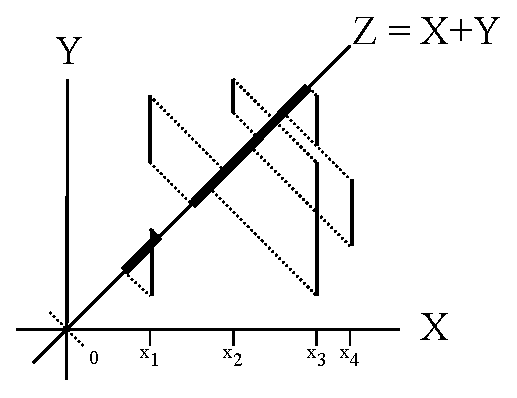
\includegraphics{Images/XY_addition_projection.eps}
  \caption[Projection of $XY$-space to $X+Y$-space]
          {Projection of $XY$-space to $X+Y$-space}
  \label{fig:XY_addition_projection}
\end{figure}

As an example suppose,

\begin{align*}
A &= \mathbf{U}(-1,2)\\
f(x) &= step(x) = \begin{cases}
0 & \text{ if x $\le$ 0},\\
1 & \text{ else}
\end{cases}\\
g(y) &= |y| + 1\\
X &= f(A)\\
Y &= g(A)
\end{align*}

then in proper form,

\begin{align*}
X &= ((0,1),(\frac{1}{3},\frac{2}{3}))\\
Y &= \mathbf{U}((0,1,2),(\frac{2}{3}, \frac{1}{3}))
\end{align*}

where $Y$ is \emph{multi-uniform} requiring probabilities within partition elements to be specified. Notice that $Pr(X = 0) = \frac{1}{3}$, $Pr(X = 1) = \frac{2}{3}$, $Pr(0 < Y < 1) = \frac{2}{3}$ and $Pr(1 < Y < 2) = \frac{1}{3}$. 

Suppose further that $Z = X+Y$. The joint $XY$ figure \ref{fig:XY_01_example} reveals the details. Noticing that the probability is uniformly distributed over the range of $XY$ and that the two fragments of that region do not overlap according to the iso-value contours of $Z$ the problem is solved by inspection so that,

\begin{align*}
Z \sim \mathbf{U}(1,4)
\end{align*}

\begin{figure}
  \centering
  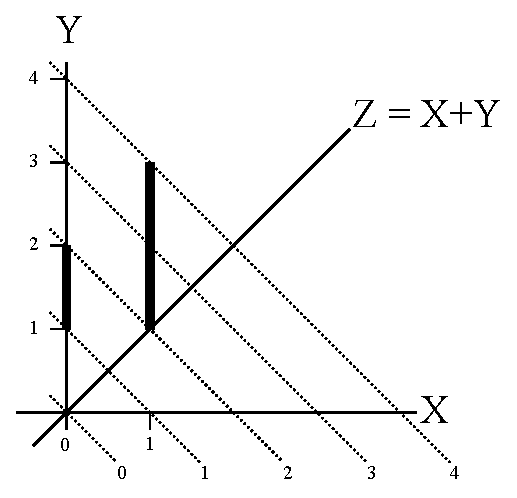
\includegraphics{Images/XY_01_example.eps}
  \caption[Example of Correlated Discrete $X$ and Continous $Y$ in $XY$-space]
          {Example of Discrete/Continous $XY$}
  \label{fig:XY_01_example}
\end{figure}

To find this result more formally $Y$ is conditioned on the discrete $X$ so that,

\begin{align*}
Y | X = 0 &\sim \mathbb{U}(1,2)\\
Y | X = 1 &\sim \mathbb{U}(1,3)
\end{align*}

then,

\begin{align*}
Z &= X + Y\\
  &= (X + Y | X = 0) \oplus (X + Y | X = 1)\\
  &= (0 + Y | X = 0) \oplus (1 + Y | X = 1)\\
  &\sim \mathbf{U}(1+0,2+0) * Pr(X = 0) + \mathbf{U}(1+1,3+1) * Pr(X = 1)\\
  &\sim \mathbf{U}(1,2) * \frac{1}{3} + \mathbf{U}(2,4) * \frac{2}{3}\\
  &\sim \mathbf{U}(1,4)
\end{align*}

For visual convenience the proper form distributions of $A$, $X$, $Y$ and $Z$ are shown in figure \ref{fig:XY_example_distributions}. Notice that to compute $Z = X + Y$ from the proper forms of $X$ and $Y$ is more challenging than from the synchronous form of $XY$ in figure \ref{fig:XY_01_example} in part because of the otherwise unseen correlation between $X$ and $Y$ through $A$.

\begin{figure}
  \centering
  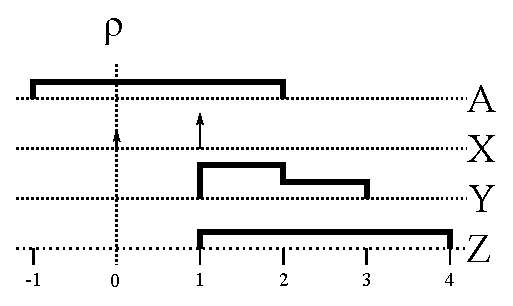
\includegraphics{Images/XY_example_distributions.eps}
  \caption[Example Discrete/Continuous Distributions in Proper Form]
          {Example Discrete/Continous Distributions in Proper Form}
  \label{fig:XY_example_distributions}
\end{figure}

%\chapter{Truncated Lognormal}
%\input{truncated_lognormal}

%%%%%%%%%%%%%%%%%%%%%%%%%%%%%%%%%%%%%%%%%%%%%%%%%%%%%%%%%%%%%%%%%%%%%%%%%%%%%%%%%%%%%%%%%%
\bibliographystyle{plain}
\bibliography{RandomVariables}
%%%%%%%%%%%%%%%%%%%%%%%%%%%%%%%%%%%%%%%%%%%%%%%%%%%%%%%%%%%%%%%%%%%%%%%%%%%%%%%%%%%%%%%%%%
\end {document}
